\providecommand{\cellpair}[5]{$\vcenter{\hbox{\begin{tikzpicture}[x=1.15em,y=1.15em]%
\node (t) at (4.2,0) {$#2$};%
\draw[->] (0.75,0.32) to[bend left=18] (3.45,0.32);%
\node at (2.1,0.88) {$\scriptstyle#3$};%

\node at (2.1,0.88) {$\scriptstyle#3$};%
\draw[->] (0.75,-0.32) to[bend right=18] (3.45,-0.32);%
\node at (2.1,-0.93) {$\scriptstyle#4$};%
\draw[->] (1.95,0.2) to[bend right=32] (1.95,-0.2);%
\node at (2.85,0) {$\scriptstyle#5$};%
\end{tikzpicture}}}$\ignorespaces}

\section{双侧纤维化}\label{sec:two-sided-fibrations}

通过分解，∞-宇宙 $\mathcal{K}$ 中任何从 $A$ 到 $B$ 的\trSpan{}都可以在%
\trEquivalence{}意义下替换为一个\textbf{双侧\trIsofibration}（two-sided
isofibration），即一个跨度 $A\xleftarrow{q}E\xrightarrow{p}B$，使得\trFunctor{}
$(q,p)\colon E\twoheadrightarrow A\times B$ 是一条\trIsofibration{}。从 $A$ 到
$B$ 的\trTwoSidedIsofibration{}，正是 ∞-宇宙 $\mathcal{K}_{A\times B}$ 中的诸对象。在本节
中，我们描述一个\trTwoSidedIsofibration{}在何种意义上是\emph{左侧余笛卡尔的}或%
\emph{右侧笛卡尔的}，然后引入\emph{\trTwoSidedFibration}，它把这两种概念整合
起来。
为了给这些概念提供动机，考虑与 ∞-宇宙 $\mathcal{K}$ 中 $A$ 的%
\trArrowInfinityCategory{}相关联的跨度 $A\xleftarrow{p_{1}}A^{2}\xrightarrow{p_{0}}A$。在命题 5.5.11 中，我们观察到
\begin{center}
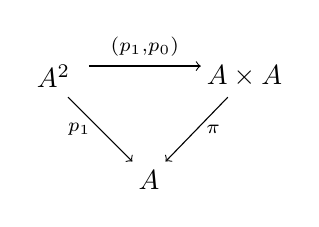
\begin{tikzpicture}[x=1.5em,y=1.5em]
  \node (A2) at (0,1.3) {$A^{2}$};
  \node (AA) at (4.6,1.3) {$A\times A$};
  \node (A)  at (2.3,-1.2) {$A$};
  \draw[->] (0.85,1.55) -- node[above]{$\scriptstyle(p_{1},p_{0})$} (3.55,1.55);
  \draw[->] (0.35,0.8) -- node[left,pos=0.5]{$\scriptstyle p_{1}$} (1.9,-0.75);
  \draw[->] (4.2,0.8) -- node[right,pos=0.5]{$\scriptstyle\pi$} (2.7,-0.75);
\end{tikzpicture}
\end{center}
定义了\trSliceInfinityCosmos{} $\mathcal{K}_{/A}$ 中的一条\trCartesianFibration%
——实际上是一条离散\trCartesianFibration{}，不过我们把对离散性的考量推迟到在
7.4 节中引入\emph{\trModule}之时。

该证明援引定理 5.2.8(iii)，它经由余定义域之上的一个\trFiberedAdjunction{}来刻画%
\trCartesianFibration{}。在此情形，该\trFiberedAdjunction{}位于 ∞-宇宙
$(\mathcal{K}_{/A})_{/\pi\colon A\times A\twoheadrightarrow A}\cong\mathcal{K}_{/A\times A}$ 之中，且等价于如下由诸指标范畴之间的一个伴随所产生的典范伴随
\begin{center}
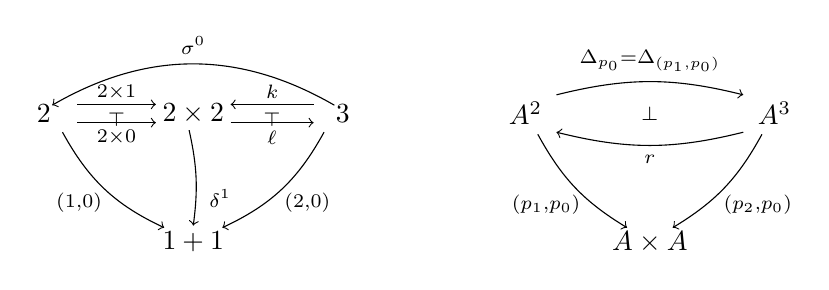
\begin{tikzpicture}[x=1.5em,y=1.5em]
  \node (two)  at (0,1.5) {$2$};
  \node (tt)   at (3.6,1.5) {$2\times 2$};
  \node (three) at (7.2,1.5) {$3$};
  \node (oo)   at (3.6,-1.6) {$1+1$};
  \draw[->] (7.0,1.7) to[bend right=30] node[above,pos=0.5]{$\scriptstyle\sigma^{0}$} (0.2,1.7);
  \draw[->] (0.8,1.72) -- (2.7,1.72);
  \node at (1.75,2.02) {$\scriptstyle 2\times 1$};
  \node at (1.75,1.36) {$\scriptstyle\top$};
  \draw[->] (0.8,1.28) -- (2.7,1.28);
  \node at (1.75,0.92) {$\scriptstyle 2\times 0$};
  \draw[->] (6.5,1.72) -- (4.5,1.72);
  \node at (5.5,2.02) {$\scriptstyle k$};
  \node at (5.5,1.36) {$\scriptstyle\top$};
  \draw[->] (4.5,1.28) -- (6.5,1.28);
  \node at (5.5,0.92) {$\scriptstyle\ell$};
  \draw[->] (0.45,1.05) to[bend right=18] (2.9,-1.25);
  \node at (0.85,-0.65) {$\scriptstyle(1,0)$};
  \draw[->] (6.75,1.05) to[bend left=18] (4.3,-1.25);
  \node at (6.35,-0.65) {$\scriptstyle(2,0)$};
  \draw[->] (3.5,1.1) to[bend left=10] (3.6,-1.2);
  \node at (4.25,-0.55) {$\scriptstyle\delta^{1}$};
  \node at (9.6,1.5) {$\twoheadrightarrow$};
  \begin{scope}[shift={(11.6,0)}]
  \node (A2)  at (0,1.5) {$A^{2}$};
  \node (A3)  at (6.0,1.5) {$A^{3}$};
  \node (AA)  at (3.0,-1.6) {$A\times A$};
  \draw[->] (0.75,1.95) to[bend left=14] node[above,pos=0.5]{$\scriptstyle\Delta_{p_{0}}=\Delta_{(p_{1},p_{0})}$} (5.25,1.95);
  \node at (3.0,1.5) {$\scriptstyle\perp$};
  \draw[->] (5.25,1.05) to[bend left=14] node[below,pos=0.5]{$\scriptstyle r$} (0.75,1.05);
  \draw[->] (0.3,1.0) to[bend right=15] (2.45,-1.25);
  \node at (0.5,-0.7) {$\scriptstyle(p_{1},p_{0})$};
  \draw[->] (5.7,1.0) to[bend left=15] (3.55,-1.25);
  \node at (5.6,-0.7) {$\scriptstyle(p_{2},p_{0})$};
  \end{scope}
\end{tikzpicture}
\end{center}
用我们即将引入的术语来说，这就是：\trTwoSidedIsofibration
$A\xleftarrow{p_{1}}A^{2}\xrightarrow{p_{0}}A$ 是\emph{右侧笛卡尔}的含义。

当我们与投向右因子的投影 $\pi\colon A\times A\twoheadrightarrow A$ 作%
\trPostComposition{}之后，便得到一个伴随
\begin{center}
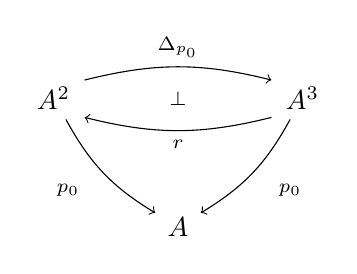
\begin{tikzpicture}[x=1.5em,y=1.5em]
  \node (A2) at (0,1.5) {$A^{2}$};
  \node (A3) at (6.0,1.5) {$A^{3}$};
  \node (A)  at (3.0,-1.6) {$A$};
  \draw[->] (0.75,1.95) to[bend left=14] node[above,pos=0.5]{$\scriptstyle\Delta_{p_{0}}$} (5.25,1.95);
  \node at (3.0,1.5) {$\scriptstyle\perp$};
  \draw[->] (5.25,1.05) to[bend left=14] node[below,pos=0.5]{$\scriptstyle r$} (0.75,1.05);
  \draw[->] (0.3,1.0) to[bend right=15] (2.45,-1.25);
  \node at (0.35,-0.7) {$\scriptstyle p_{0}$};
  \draw[->] (5.7,1.0) to[bend left=15] (3.55,-1.25);
  \node at (5.7,-0.7) {$\scriptstyle p_{0}$};
\end{tikzpicture}
\end{center}
它见证了命题 5.2.9 所确立的事实：$p_{0}\colon A^{2}\twoheadrightarrow A$ 是一条%
\trCartesianFibration{}。因此，说一个\trTwoSidedIsofibration{}是右侧笛卡尔的，其一部分含义
便是：它的右腿是一条\trCartesianFibration{}。说这个伴随位于 $A\times A$ 之上而不
仅仅位于 $A$ 之上，则等价于断言：$p_{0}$-笛卡尔提升可以选取得落在
$p_{1}\colon A^{2}\twoheadrightarrow A$ 的诸\trFiber{}之中，并且沿左腿须化后
成为恒同箭头。由此可知，每支 $p_{0}$-笛卡尔变换与 $p_{1}$ 须化后都是一个%
\trIsomorphism{}。

这两条性质还有另一种表达方式：即要求\trFunctor{}
\begin{center}
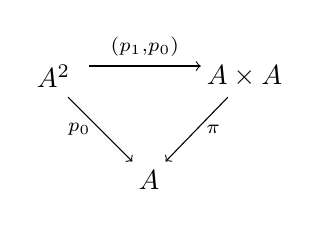
\begin{tikzpicture}[x=1.5em,y=1.5em]
  \node (A2) at (0,1.3) {$A^{2}$};
  \node (AA) at (4.6,1.3) {$A\times A$};
  \node (A)  at (2.3,-1.2) {$A$};
  \draw[->] (0.85,1.55) -- node[above]{$\scriptstyle(p_{1},p_{0})$} (3.55,1.55);
  \draw[->] (0.35,0.8) -- node[left,pos=0.5]{$\scriptstyle p_{0}$} (1.9,-0.75);
  \draw[->] (4.2,0.8) -- node[right,pos=0.5]{$\scriptstyle\pi$} (2.7,-0.75);
\end{tikzpicture}
\end{center}
落在 ∞-宇宙 $\mathcal{C}art(\mathcal{K})_{/A}\subset\mathcal{K}_{/A}$ 之中。
这首先断言 $p_{0}\colon A^{2}\twoheadrightarrow A$ 是一条\trCartesianFibration{}，
其次断言 $(p_{1},p_{0})$ 定义了从这个\trCartesianFibration{}到例 5.4.6 的%
\trCartesianFibration{} $\pi\colon A\times A\twoheadrightarrow A$ 的一个笛卡尔
函子。正如彼处所观察到的，诸 $\pi$-笛卡尔胞腔正是那些与另一个投影须化后成为%
\trIsomorphism{}的\trNaturalTransformation{}。于是，说 $(p_{1},p_{0})$ 是
一个\trCartesianFunctor{}，恰好就是说 $p_{1}$ 把诸 $p_{0}$-笛卡尔变换都送到\trIsomorphism{}。

我们现在把这些直觉形式化：

\begin{lemma}[右侧笛卡尔的]\label{lem:cartesian-on-the-right}
设 $A\xleftarrow{q}E\xrightarrow{p}B$ 是 ∞-宇宙 $\mathcal{K}$ 中的一个双侧等价
纤维化，则下列诸条等价：
\begin{enumerate}[label=(\roman*)]
\item \trFunctor{}
\begin{center}
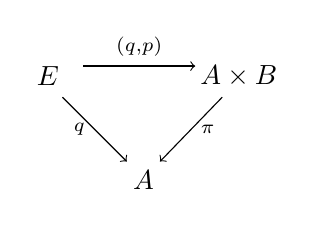
\begin{tikzpicture}[x=1.5em,y=1.5em]
  \node (E)  at (0,1.3) {$E$};
  \node (AB) at (4.6,1.3) {$A\times B$};
  \node (A)  at (2.3,-1.2) {$A$};
  \draw[->] (0.85,1.55) -- node[above]{$\scriptstyle(q,p)$} (3.55,1.55);
  \draw[->] (0.35,0.8) -- node[left,pos=0.5]{$\scriptstyle q$} (1.9,-0.75);
  \draw[->] (4.2,0.8) -- node[right,pos=0.5]{$\scriptstyle\pi$} (2.7,-0.75);
\end{tikzpicture}
\end{center}
是\trSliceInfinityCosmos{} $\mathcal{K}_{/A}$ 中的一条\trCartesianFibration{}。
\item \trFunctor{}
\begin{center}
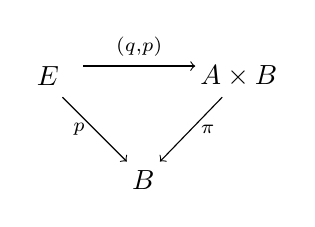
\begin{tikzpicture}[x=1.5em,y=1.5em]
  \node (E)  at (0,1.3) {$E$};
  \node (AB) at (4.6,1.3) {$A\times B$};
  \node (B)  at (2.3,-1.2) {$B$};
  \draw[->] (0.85,1.55) -- node[above]{$\scriptstyle(q,p)$} (3.55,1.55);
  \draw[->] (0.35,0.8) -- node[left,pos=0.5]{$\scriptstyle p$} (1.9,-0.75);
  \draw[->] (4.2,0.8) -- node[right,pos=0.5]{$\scriptstyle\pi$} (2.7,-0.75);
\end{tikzpicture}
\end{center}
在 $\mathcal{K}_{/B}$ 中落在子 ∞-宇宙 $\mathcal{C}art(\mathcal{K})_{/B}$ 之中。
\item 由 $\mathrm{id}_{p}$ 诱导的\trFunctor{}在 $\mathcal{K}_{/A\times B}$ 中
容有一个\trRightAdjoint{}：
\begin{center}
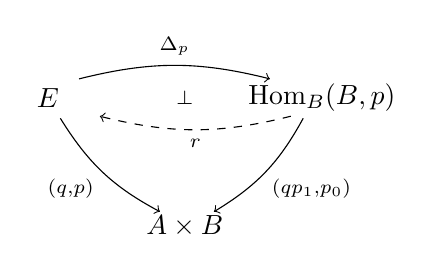
\begin{tikzpicture}[x=1.5em,y=1.5em]
  \node (E)   at (0,1.5) {$E$};
  \node (Hom) at (6.6,1.5) {$\mathrm{Hom}_{B}(B,p)$};
  \node (AB)  at (3.3,-1.6) {$A\times B$};
  \draw[->] (0.75,1.95) to[bend left=14] node[above,pos=0.5]{$\scriptstyle\Delta_{p}$} (5.35,1.95);
  \node at (3.3,1.5) {$\scriptstyle\perp$};
  \draw[->,dashed] (5.85,1.05) to[bend left=14] node[below,pos=0.5]{$\scriptstyle r$} (1.25,1.05);
  \draw[->] (0.3,1.0) to[bend right=15] (2.7,-1.25);
  \node at (0.55,-0.7) {$\scriptstyle(q,p)$};
  \draw[->] (6.15,1.0) to[bend left=15] (4.0,-1.25);
  \node at (6.35,-0.7) {$\scriptstyle(qp_{1},p_{0})$};
\end{tikzpicture}
\end{center}
\item 等价纤维化 $p\colon E\twoheadrightarrow B$ 是 $\mathcal{K}$ 中的一条%
\trCartesianFibration{}，并且对每支 $p$-笛卡尔变换
\cellpair{X}{E}{e'}{e}{\psi\psi}，其须化复合
\cellpair{X}{E}{e'}{e}{\psi\psi} $E\xrightarrow{q}A$
是一个\trIsomorphism{}。
\end{enumerate}
一个\trTwoSidedIsofibration $A\xleftarrow{q}E\xrightarrow{p}B$ 称为\textbf{右侧笛卡尔的}
（cartesian on the right），当这些等价条件被满足时。
\end{lemma}

\begin{proof}
等价 $(i)\Leftrightarrow(iii)$ 恰好是把定理 5.2.8(i)$\Leftrightarrow$(iii)
应用于\trSliceInfinityCosmos{} $\mathcal{K}_{/A}$ 中的等价纤维化
$(q,p)\colon E\twoheadrightarrow A\times B$ 而得的解读。后一结果断言：%
$\mathcal{K}_{/A}$ 中的等价纤维化 $(q,p)\colon E\twoheadrightarrow A\times B$
是一条\trCartesianFibration{}，当且仅当由 $\mathrm{id}_{(q,p)}$ 诱导的、从 $E$ 到%
\trFunctor{} $(q,p)\colon E\twoheadrightarrow A\times B$ 之右表示的那个%
\trFunctor{}容有一个余定义域 $\pi\colon A\times B\twoheadrightarrow A$ 之上的%
\trRightAdjoint{}；由于
$(\mathcal{K}_{/A})_{/\pi\colon A\times B\twoheadrightarrow A}\cong\mathcal{K}_{/A\times B}$，这与在 $A\times B$ 之上断言该伴随是一回事。

在 $\mathcal{K}_{/A}$ 中解读定理 5.2.8 的唯一微妙之处，在于为\trFunctor{}
$(q,p)\colon E\twoheadrightarrow A\times B$ 正确解读 $\mathcal{K}_{/A}$ 中的左
可表示\trCommaInfinityCategory{}。这个\trCommaInfinityCategory{}被构造为 $\mathcal{K}_{/A}$
中对象 $\pi\colon A\times B\to A$ 的 2-\trCotensor{}的一个\trSubobject{}，而命题
1.2.22 告诉我们，后者作为如下拉回方图的左侧竖直边而形成
\begin{center}
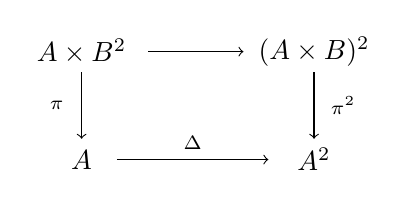
\begin{tikzpicture}[x=1.5em,y=1.5em]
  \node (AB2)  at (0,1.3) {$A\times B^{2}$};
  \node (AB2s) at (5.6,1.3) {$(A\times B)^{2}$};
  \node (A)    at (0,-1.3) {$A$};
  \node (A2)   at (5.6,-1.3) {$A^{2}$};
  \draw[->] (1.6,1.3) -- (3.9,1.3);
  \draw[->] (0,0.8) -- (0,-0.8);  \node at (-0.6,0) {$\scriptstyle\pi$};
  \draw[->] (5.6,0.8) -- (5.6,-0.8);  \node at (6.3,0) {$\scriptstyle\pi^{2}$};
  \draw[->] (0.85,-1.3) -- node[above]{$\scriptstyle\Delta$} (4.5,-1.3);
  \node at (0.55,0.75) {$\scriptstyle\llcorner$};
\end{tikzpicture}
\end{center}
按 (3.4.2)，这个\trCommaInfinityCategory{}由 $\mathcal{K}_{/A}$ 中的如下拉回
构造
\begin{rveq}\label{eq:slice-comma-pullback}
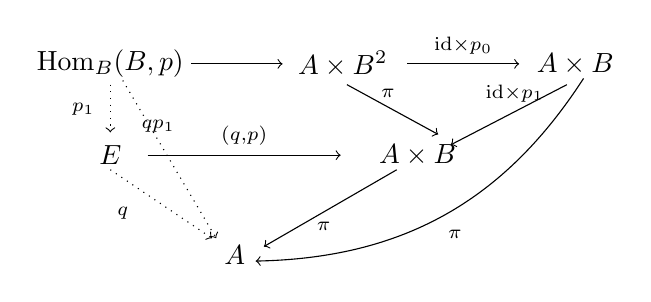
\begin{tikzpicture}[x=1.5em,y=1.5em]
  \node (Hom) at (0,2.6) {$\mathrm{Hom}_{B}(B,p)$};
  \node (AB2) at (5.6,2.6) {$A\times B^{2}$};
  \node (ABt) at (11.2,2.6) {$A\times B$};
  \node (E)   at (0,0.4) {$E$};
  \node (ABm) at (7.4,0.4) {$A\times B$};
  \node (A)   at (3.0,-2.0) {$A$};
  \draw[->] (1.95,2.6) -- (4.15,2.6);
  \draw[->] (7.15,2.6) -- node[above]{$\scriptstyle\mathrm{id}\times p_{0}$} (9.85,2.6);
  \draw[->,dotted] (0,2.1) -- (0,0.95);
  \node at (-0.65,1.5) {$\scriptstyle p_{1}$};
  \draw[->,dotted] (0.3,2.2) -- (2.55,-1.6);
  \node at (1.15,1.1) {$\scriptstyle qp_{1}$};
  \node at (0.55,2.3) {$\scriptstyle\lrcorner$};
  \draw[->] (5.7,2.1) -- node[above,pos=0.45]{$\scriptstyle\pi$} (7.9,0.9);
  \draw[->] (11.0,2.1) -- node[above,pos=0.45]{$\scriptstyle\mathrm{id}\times p_{1}$} (8.2,0.65);
  \draw[->] (0.9,0.4) -- node[above,pos=0.5]{$\scriptstyle(q,p)$} (5.55,0.4);
  \draw[->,dotted] (0,0.05) -- (2.45,-1.6);
  \node at (0.3,-1.0) {$\scriptstyle q$};
  \draw[->] (6.9,0.05) -- node[below,pos=0.55]{$\scriptstyle\pi$} (3.7,-1.8);
  \draw[->] (11.4,2.25) to[bend left=28] (3.5,-2.15);
  \node at (8.3,-1.5) {$\scriptstyle\pi$};
\end{tikzpicture}
\end{rveq}
该拉回由遗忘\trFunctor{} $\mathcal{K}_{/A}\to\mathcal{K}$ 所创造，且其余定义域
投影函子是顶部复合
$(qp_{1},p_{0})\colon\mathrm{Hom}_{B}(B,p)\twoheadrightarrow A\times B$。现在
我们看到，定理 5.2.8(i)$\Leftrightarrow$(iii) 在 $\mathcal{K}_{/A}$ 中的解读
恰好就是等价 $(i)\Leftrightarrow(iii)$。

剩下要论证的是与 (ii) 和 (iv) 的等价。假设 (iii) 并与
$\pi\colon A\times B\twoheadrightarrow B$ 复合，便得到一个\trFiberedAdjunction，后者证明
$p$ 是一条\trCartesianFibration{}。这两个\trFiberedAdjunction{}的\trCounit{}是同一个，并且由
定理 5.2.8(iii)，复合
\begin{center}
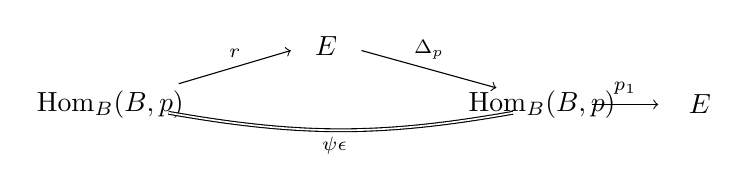
\begin{tikzpicture}[x=1.5em,y=1.5em]
  \node (H1) at (0,0) {$\mathrm{Hom}_{B}(B,p)$};
  \node (E)  at (5.2,1.4) {$E$};
  \node (H2) at (10.4,0) {$\mathrm{Hom}_{B}(B,p)$};
  \node (E2) at (14.2,0) {$E$};
  \draw[->] (1.65,0.5) -- node[above,pos=0.5]{$\scriptstyle r$} (4.35,1.3);
  \draw[->] (6.05,1.3) -- node[above,pos=0.5]{$\scriptstyle\Delta_{p}$} (9.3,0.4);
  \draw[double] (1.4,-0.2) to[bend right=10] (9.7,-0.2);
  \node at (5.4,-1.0) {$\scriptstyle\psi\epsilon$};
  \draw[->] (11.6,0) -- node[above,pos=0.5]{$\scriptstyle p_{1}$} (13.2,0);
\end{tikzpicture}
\end{center}
是泛 $p$-笛卡尔胞腔。由于 $\epsilon$ 在 $A\times B$ 之上纤维化，与 $q$ 作后
复合后便得到一个恒同，这就告诉我们 $q\colon E\twoheadrightarrow A$ 把诸 $p$-笛卡尔胞腔都送到%
\trIsomorphism{}。这证明了 (iii) 蕴涵 (iv)。

由例 5.4.6，\trCartesianFibration{} $\pi\colon A\times B\twoheadrightarrow B$
的诸笛卡尔胞腔恰好是那些余定义域为 $A$ 的分量为\trIsomorphism{}的 2-\trCell{}，
因此 (iv) 恰好说 $(q,p)\colon E\twoheadrightarrow A\times B$ 定义了从 $p$ 到
$\pi$ 的一个\trCartesianFunctor{}。于是 (iv) 蕴涵 (ii)。

为完成论证，我们来证明 (ii) 蕴涵 (i)。假设 (ii) 并考虑 $\mathcal{K}_{/A}$ 中的
一个 2-\trCell
\begin{center}
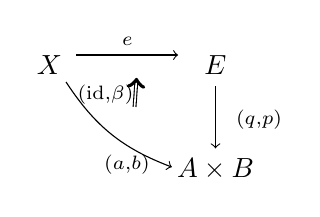
\begin{tikzpicture}[x=1.5em,y=1.5em]
  \node (X)  at (0,1.3) {$X$};
  \node (E)  at (4.0,1.3) {$E$};
  \node (AB) at (4.0,-1.2) {$A\times B$};
  \draw[->] (0.65,1.55) -- node[above]{$\scriptstyle e$} (3.1,1.55);
  \draw[->] (4.0,0.8) -- (4.0,-0.7);
  \node at (5.05,0) {$\scriptstyle(q,p)$};
  \draw[->] (0.4,0.9) to[bend right=18] node[below,pos=0.65]{$\scriptstyle(a,b)$} (2.95,-1.15);
  \draw[double,->] (2.05,0.3) -- (2.1,1.0);
  \node at (1.35,0.6) {$\scriptstyle(\mathrm{id},\beta)$};
\end{tikzpicture}
\end{center}
由于 $p$ 是一条\trCartesianFibration{}，$\beta\colon b\Rightarrow pe$ 容有一个
$p$-笛卡尔提升 $\chi\colon e'\Rightarrow e$；又由于 $(q,p)$ 是一个\trCartesianFunctor{}，
须化后的 2-\trCell{} $q\chi\colon qe'\Rightarrow a$ 是一个\trIsomorphism{}。由于
$(q,p)\colon E\twoheadrightarrow A\times B$ 是一条\trIsofibration{}，我们可以把
2-\trCell{} $(q\chi^{-1},\mathrm{id})\colon(a,b)\Rightarrow e'$ 提升为一个可逆
2-\trCell{} $\gamma\colon e''\Rightarrow e'$，满足 $p\gamma=\mathrm{id}_{b}$。
复合 $\chi\cdot\gamma\colon e''\Rightarrow e$ 是 $(\mathrm{id},\beta)$ 沿
$(q,p)$ 在 $A$ 之上的一个提升，且容易验证：它满足命题 5.2.11 所确立的、刻画
$\mathcal{K}_{/A}$ 中 $(\mathrm{id},\beta)$ 的 $(q,p)$-笛卡尔提升的那些弱%
\trUniversalProperty{}。这就证明了 (i)。
\end{proof}

合并\cref{lem:cartesian-on-the-right}及其对偶——后者定义了\textbf{左侧余笛卡尔的}
（cocartesian on the left）那类\trTwoSidedIsofibration——便得到：

\begin{corollary}\label{cor:cartesian-cocartesian-conditions}
∞-宇宙 $\mathcal{K}$ 中的一个\trTwoSidedIsofibration
$A\xleftarrow{q}E\xrightarrow{p}B$ 是左侧余笛卡尔的且是右侧笛卡尔的，若下列诸
等价条件被满足：
\begin{enumerate}[label=(\roman*)]
\item \trFunctor{}
\begin{center}
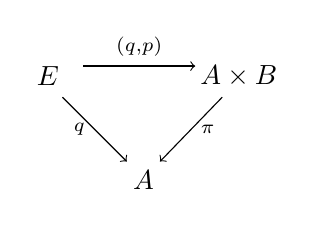
\begin{tikzpicture}[x=1.5em,y=1.5em]
  \node (E)  at (0,1.3) {$E$};
  \node (AB) at (4.6,1.3) {$A\times B$};
  \node (A)  at (2.3,-1.2) {$A$};
  \draw[->] (0.85,1.55) -- node[above]{$\scriptstyle(q,p)$} (3.55,1.55);
  \draw[->] (0.35,0.8) -- node[left,pos=0.5]{$\scriptstyle q$} (1.9,-0.75);
  \draw[->] (4.2,0.8) -- node[right,pos=0.5]{$\scriptstyle\pi$} (2.7,-0.75);
\end{tikzpicture}
\end{center}
落在 $\mathrm{co}\mathcal{C}\mathit{art}(\mathcal{K})_{/A}$ 之中，并定义 $\mathcal{K}_{/A}$
中的一条\trCartesianFibration{}。
\item \trFunctor{}
\begin{center}
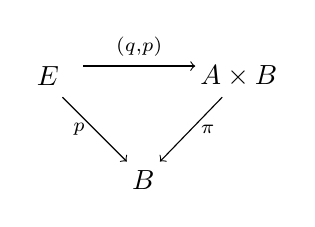
\begin{tikzpicture}[x=1.5em,y=1.5em]
  \node (E)  at (0,1.3) {$E$};
  \node (AB) at (4.6,1.3) {$A\times B$};
  \node (B)  at (2.3,-1.2) {$B$};
  \draw[->] (0.85,1.55) -- node[above]{$\scriptstyle(q,p)$} (3.55,1.55);
  \draw[->] (0.35,0.8) -- node[left,pos=0.5]{$\scriptstyle p$} (1.9,-0.75);
  \draw[->] (4.2,0.8) -- node[right,pos=0.5]{$\scriptstyle\pi$} (2.7,-0.75);
\end{tikzpicture}
\end{center}
落在 $\mathcal{C}art(\mathcal{K})_{/B}$ 之中，并定义 $\mathcal{K}_{/B}$ 中的一
条\trCocartesianFibration{}。
\end{enumerate}
\end{corollary}

一个\emph{\trTwoSidedFibration}是一个如下跨度：它左侧余笛卡尔、右侧笛卡尔，
并且满足一条进一步的相容性条件——该条件可以用若干种等价的方式来陈述，而这些
陈述归结为断言：取 $q$-余笛卡尔提升与取 $p$-笛卡尔提升这两个过程相互交换：

\begin{theorem}\label{thm:two-sided-fibration}
设 $A\xleftarrow{q}E\xrightarrow{p}B$ 是 ∞-宇宙 $\mathcal{K}$ 中的一个双侧等价
纤维化，则下列诸条等价：
\begin{enumerate}[label=(\roman*)]
\item \trFunctor{}
\begin{center}
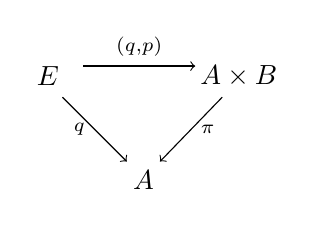
\begin{tikzpicture}[x=1.5em,y=1.5em]
  \node (E)  at (0,1.3) {$E$};
  \node (AB) at (4.6,1.3) {$A\times B$};
  \node (A)  at (2.3,-1.2) {$A$};
  \draw[->] (0.85,1.55) -- node[above]{$\scriptstyle(q,p)$} (3.55,1.55);
  \draw[->] (0.35,0.8) -- node[left,pos=0.5]{$\scriptstyle q$} (1.9,-0.75);
  \draw[->] (4.2,0.8) -- node[right,pos=0.5]{$\scriptstyle\pi$} (2.7,-0.75);
\end{tikzpicture}
\end{center}
定义了 $\mathrm{co}\mathcal{C}\mathit{art}(\mathcal{K})_{/A}$ 中的一条\trCartesianFibration{}。
\item \trFunctor{}
\begin{center}
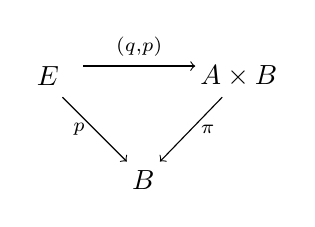
\begin{tikzpicture}[x=1.5em,y=1.5em]
  \node (E)  at (0,1.3) {$E$};
  \node (AB) at (4.6,1.3) {$A\times B$};
  \node (B)  at (2.3,-1.2) {$B$};
  \draw[->] (0.85,1.55) -- node[above]{$\scriptstyle(q,p)$} (3.55,1.55);
  \draw[->] (0.35,0.8) -- node[left,pos=0.5]{$\scriptstyle p$} (1.9,-0.75);
  \draw[->] (4.2,0.8) -- node[right,pos=0.5]{$\scriptstyle\pi$} (2.7,-0.75);
\end{tikzpicture}
\end{center}
定义了 $\mathcal{C}art(\mathcal{K})_{/B}$ 中的一条\trCocartesianFibration{}。
\item 诸典范\trFunctor{}在 $\mathcal{K}_{/A\times B}$ 中容有如下所示的诸伴随
\begin{center}
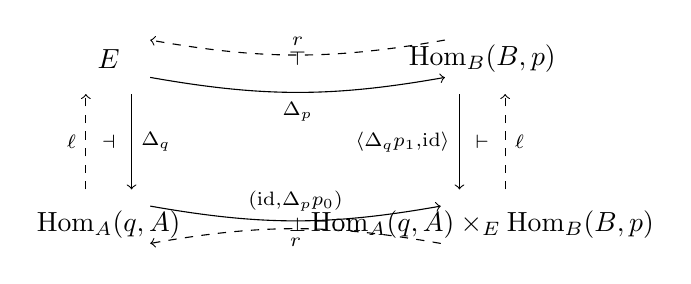
\begin{tikzpicture}[x=1.5em,y=1.5em]
  \node (E)    at (0,2.3) {$E$};
  \node (HomB) at (9.0,2.3) {$\mathrm{Hom}_{B}(B,p)$};
  \node (HomA) at (0,-1.7) {$\mathrm{Hom}_{A}(q,A)$};
  \node (P)    at (9.0,-1.7)
    {$\mathrm{Hom}_{A}(q,A)\times_{E}\mathrm{Hom}_{B}(B,p)$};
  \draw[->,dashed] (8.1,2.75) to[bend left=10] node[above,pos=0.5]{$\scriptstyle r$} (1.0,2.75);
  \node at (4.55,2.3) {$\scriptstyle\top$};
  \draw[->] (1.0,1.85) to[bend right=10] node[below,pos=0.5]{$\scriptstyle\Delta_{p}$} (8.1,1.85);
  \draw[->,dashed] (-0.55,-0.85) -- node[left,pos=0.5]{$\scriptstyle\ell$} (-0.55,1.45);
  \node at (0,0.3) {$\scriptstyle\dashv$};
  \draw[->] (0.55,1.45) -- node[right,pos=0.5]{$\scriptstyle\Delta_{q}$} (0.55,-0.85);
  \draw[->] (8.45,1.45) -- node[left,pos=0.5]{$\scriptstyle\langle\Delta_{q}p_{1},\mathrm{id}\rangle$} (8.45,-0.85);
  \node at (9.0,0.3) {$\scriptstyle\vdash$};
  \draw[->,dashed] (9.55,-0.85) -- node[right,pos=0.5]{$\scriptstyle\ell$} (9.55,1.45);
  \draw[->] (1.0,-1.25) to[bend right=10] node[above,pos=0.5]{$\scriptstyle(\mathrm{id},\Delta_{p}p_{0})$} (8.0,-1.25);
  \node at (4.55,-1.7) {$\scriptstyle\perp$};
  \draw[->,dashed] (8.0,-2.15) to[bend right=10] node[below,pos=0.5]{$\scriptstyle r$} (1.0,-2.15);
\end{tikzpicture}
\end{center}
并且该所示交换方块中恒同 2-胞腔的对应定义出一个同构 $\ell r\cong r\ell$。
\item \trTwoSidedIsofibration $A\xleftarrow{q}E\xrightarrow{p}B$ 是左侧余笛卡尔的、右侧
笛卡尔的，并且满足下述进一步的条件：给定如下左图所示的任一对%
\trNaturalTransformation{} $\alpha\colon qe\Rightarrow a$、
$\beta\colon b\Rightarrow pe$，以及如下右图所示的、$\alpha$ 在 $B$ 之上的
$q$-余笛卡尔提升 $\psi\colon e\Rightarrow\alpha_{*}e$ 与 $\beta$ 在 $A$ 之上的
$p$-笛卡尔提升 $\chi\colon\beta^{*}e\Rightarrow e$：
\begin{center}
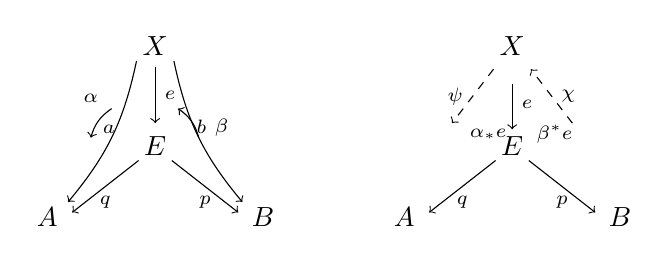
\begin{tikzpicture}[x=1.5em,y=1.5em]
  \begin{scope}[shift={(0,0)}]
  \node (X) at (2.6,1.5) {$X$};
  \node (E) at (2.6,-0.9) {$E$};
  \node (A) at (0,-2.6) {$A$};
  \node (B) at (5.2,-2.6) {$B$};
  \draw[->] (2.6,1.0) -- node[right,pos=0.5]{$\scriptstyle e$} (2.6,-0.35);
  \draw[->] (2.2,-1.25) -- node[below]{$\scriptstyle q$} (0.6,-2.5);
  \draw[->] (3.0,-1.25) -- node[below]{$\scriptstyle p$} (4.6,-2.5);
  \draw[->] (2.15,1.15) to[bend left=14] node[above,pos=0.55]{$\scriptstyle a$} (0.5,-2.25);
  \draw[->] (3.05,1.15) to[bend right=14] node[above,pos=0.55]{$\scriptstyle b$} (4.7,-2.25);
  \draw[->] (1.55,0.0) to[bend right=20] (1.05,-0.7);
  \node at (1.05,0.25) {$\scriptstyle\alpha$};
  \draw[->] (3.65,-0.7) to[bend right=20] (3.15,0.0);
  \node at (4.2,-0.45) {$\scriptstyle\beta$};
  \end{scope}
  \node at (7.3,-0.6) {$\twoheadrightarrow$};
  \begin{scope}[shift={(8.6,0)}]
  \node (X) at (2.6,1.5) {$X$};
  \node (E) at (2.6,-0.9) {$E$};
  \node (A) at (0,-2.6) {$A$};
  \node (B) at (5.2,-2.6) {$B$};
  \draw[->,dashed] (2.15,0.95) -- node[left,pos=0.5]{$\scriptstyle\psi$} (1.15,-0.35);
  \node at (2.02,-0.62) {$\scriptstyle\alpha_{*}e$};
  \draw[->] (2.6,0.6) -- node[right,pos=0.45]{$\scriptstyle e$} (2.6,-0.5);
  \draw[->,dashed] (4.05,-0.35) -- node[right,pos=0.5]{$\scriptstyle\chi$} (3.05,0.95);
  \node at (3.62,-0.62) {$\scriptstyle\beta^{*}e$};
  \draw[->] (2.2,-1.25) -- node[below]{$\scriptstyle q$} (0.6,-2.5);
  \draw[->] (3.0,-1.25) -- node[below]{$\scriptstyle p$} (4.6,-2.5);
  \end{scope}
\end{tikzpicture}
\end{center}
那么就存在一个在 $A\times B$ 之上的同构
$\alpha_{*}\beta^{*}e\cong\beta^{*}\alpha_{*}e$，它与 $\alpha\cdot q\chi$ 在
$B$ 之上的 $q$-余笛卡尔提升以及 $p\psi\cdot\beta$ 在 $A$ 之上的 $p$-笛卡尔提升
相交换：
\begin{center}
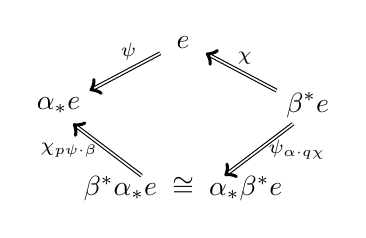
\begin{tikzpicture}[x=1.5em,y=1.5em]
  \node (e)    at (3.4,1.9) {$e$};
  \node (ase)  at (0.4,0.4) {$\alpha_{*}e$};
  \node (bse)  at (6.4,0.4) {$\beta^{*}e$};
  \node (bot)  at (3.4,-1.6) {$\beta^{*}\alpha_{*}e\;\cong\;\alpha_{*}\beta^{*}e$};
  \draw[double,->] (2.85,1.65) -- node[above,pos=0.45]{$\scriptstyle\psi$} (1.15,0.75);
  \draw[double,->] (5.65,0.75) -- node[above,pos=0.45]{$\scriptstyle\chi$} (3.95,1.65);
  \draw[double,->] (2.4,-1.3) -- node[left,pos=0.5]{$\scriptstyle\chi_{p\psi\cdot\beta}$} (0.75,-0.05);
  \draw[double,->] (6.05,-0.05) -- node[right,pos=0.5]{$\scriptstyle\psi_{\alpha\cdot q\chi}$} (4.4,-1.3);
\end{tikzpicture}
\end{center}
\end{enumerate}
当一个\trTwoSidedIsofibration $A\xleftarrow{q}E\xrightarrow{p}B$ 满足这些等价条件时，
它就定义了一个从 $A$ 到 $B$ 的\textbf{\trTwoSidedFibration}（two-sided
fibration）。
\end{theorem}

\begin{proof}
我们的策略是证明条件 (i) 等价于 (iii)——在切片 ∞-宇宙
$\mathcal{K}_{/A\times B}$ 中一个由等式见证的条件。对偶的论证表明条件 (ii)
等价于 (iii)。然后我们解析这个条件，以证明它与 (iv) 的等价。
若 (i) 成立，则 $A\xleftarrow{q}E\xrightarrow{p}B$ 也满足%
\cref{cor:cartesian-cocartesian-conditions}的条件 (i)，因为作为%
\trCartesianFibration{}这一性质被宇宙论\trFunctor{}
$\mathrm{co}\mathcal{C}\mathit{art}(\mathcal{K})_{/A}\hookrightarrow\mathcal{K}_{/A}$
所保持。于是 $A\xleftarrow{q}E\xrightarrow{p}B$ 特别地左侧余笛卡尔且右侧
笛卡尔，从而配备有伴随
\begin{center}
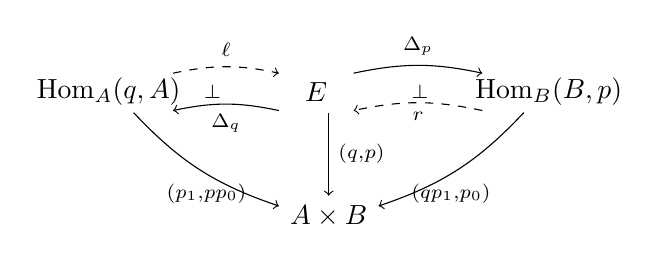
\begin{tikzpicture}[x=1.5em,y=1.5em]
  \node (HomA) at (0,1.5) {$\mathrm{Hom}_{A}(q,A)$};
  \node (E)    at (5.0,1.5) {$E$};
  \node (HomB) at (10.6,1.5) {$\mathrm{Hom}_{B}(B,p)$};
  \node (AB)   at (5.3,-1.5) {$A\times B$};
  \draw[->,dashed] (1.55,1.95) to[bend left=12] node[above,pos=0.5]{$\scriptstyle\ell$} (4.1,1.95);
  \node at (2.5,1.5) {$\scriptstyle\perp$};
  \draw[->] (4.1,1.05) to[bend right=12] node[below,pos=0.5]{$\scriptstyle\Delta_{q}$} (1.55,1.05);
  \draw[->] (5.9,1.95) to[bend left=12] node[above,pos=0.5]{$\scriptstyle\Delta_{p}$} (9.0,1.95);
  \node at (7.5,1.5) {$\scriptstyle\perp$};
  \draw[->,dashed] (9.0,1.05) to[bend right=12] node[below,pos=0.5]{$\scriptstyle r$} (5.9,1.05);
  \draw[->] (0.6,1.0) to[bend right=14] node[below,pos=0.55]{$\scriptstyle(p_{1},pp_{0})$} (4.1,-1.25);
  \draw[->] (5.3,1.0) -- node[right,pos=0.5]{$\scriptstyle(q,p)$} (5.3,-1.0);
  \draw[->] (10.0,1.0) to[bend left=14] node[below,pos=0.55]{$\scriptstyle(qp_{1},p_{0})$} (6.5,-1.25);
\end{tikzpicture}
\end{center}
由引理 3.6.6，我们可以把左手边的伴随沿
$A\times p_{1}\colon A\times B^{2}\twoheadrightarrow A\times B$ 拉回、再与
$A\times p_{0}\colon A\times B^{2}\twoheadrightarrow A\times B$ 复合，以得到下方右手边的%
\trFiberedAdjunction；并且同样把右手边的伴随沿
$p_{0}\times B\colon A^{2}\times B\twoheadrightarrow A\times B$ 拉回、再与
$p_{1}\times B\colon A^{2}\times B\twoheadrightarrow A\times B$ 复合，以得到下方左手边的%
\trFiberedAdjunction：
\begin{center}
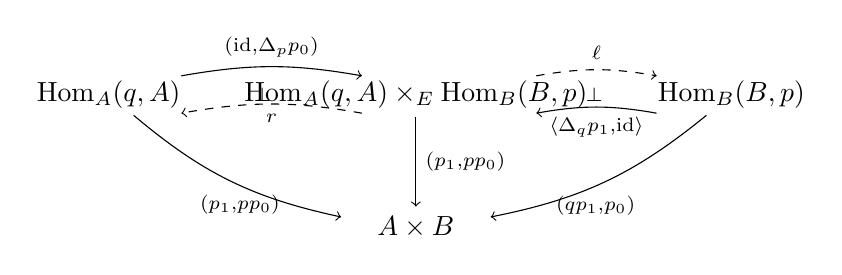
\begin{tikzpicture}[x=1.5em,y=1.5em]
  \node (HomA) at (0,1.5) {$\mathrm{Hom}_{A}(q,A)$};
  \node (P)    at (7.4,1.5)
    {$\mathrm{Hom}_{A}(q,A)\times_{E}\mathrm{Hom}_{B}(B,p)$};
  \node (HomB) at (15.0,1.5) {$\mathrm{Hom}_{B}(B,p)$};
  \node (AB)   at (7.4,-1.7) {$A\times B$};
  \draw[->] (1.75,1.95) to[bend left=10] node[above,pos=0.5]{$\scriptstyle(\mathrm{id},\Delta_{p}p_{0})$} (6.1,1.95);
  \node at (3.7,1.5) {$\scriptstyle\perp$};
  \draw[->,dashed] (6.1,1.05) to[bend right=10] node[below,pos=0.5]{$\scriptstyle r$} (1.75,1.05);
  \draw[->,dashed] (10.3,1.95) to[bend left=10] node[above,pos=0.5]{$\scriptstyle\ell$} (13.2,1.95);
  \node at (11.7,1.5) {$\scriptstyle\perp$};
  \draw[->] (13.2,1.05) to[bend right=10] node[below,pos=0.5]{$\scriptstyle\langle\Delta_{q}p_{1},\mathrm{id}\rangle$} (10.3,1.05);
  \draw[->] (7.4,0.95) -- node[right,pos=0.5]{$\scriptstyle(p_{1},pp_{0})$} (7.4,-1.2);
  \draw[->] (0.6,1.0) to[bend right=14] node[below,pos=0.55]{$\scriptstyle(p_{1},pp_{0})$} (5.6,-1.45);
  \draw[->] (14.4,1.0) to[bend left=14] node[below,pos=0.55]{$\scriptstyle(qp_{1},p_{0})$} (9.2,-1.45);
\end{tikzpicture}
\end{center}
尚待说明的是 (i) 中的假设——$(q,p)$ 定义
$\mathrm{co}\mathcal{C}\mathit{art}(\mathcal{K})_{/A}$ 中、而非仅仅 $\mathcal{K}_{/A}$
中的一条\trCartesianFibration{}。由定理 5.2.8(iii)，这个附加条件等价于断言：
右伴随
\begin{center}
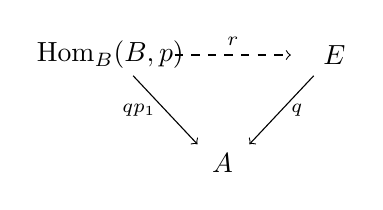
\begin{tikzpicture}[x=1.5em,y=1.5em]
  \node (Hom) at (0,1.3) {$\mathrm{Hom}_{B}(B,p)$};
  \node (E)   at (5.4,1.3) {$E$};
  \node (A)   at (2.7,-1.3) {$A$};
  \draw[->,dashed] (1.55,1.3) -- node[above]{$\scriptstyle r$} (4.35,1.3);
  \draw[->] (0.55,0.8) -- node[left,pos=0.5]{$\scriptstyle qp_{1}$} (2.1,-0.85);
  \draw[->] (4.9,0.8) -- node[right,pos=0.5]{$\scriptstyle q$} (3.35,-0.85);
\end{tikzpicture}
\end{center}
定义了从余笛卡尔纤维化 $p_{1}$ 到余笛卡尔纤维化 $q$ 的一个\trCartesianFunctor{}。由定理
5.3.4(iii)，这等价于断言：实线箭头方块
中同构的对应\footnote{实线箭头方块中的这个同构，是见证「$\Delta_{q}$ 定义了从
$p$ 到 $p_{0}$ 的一个\trCartesianFunctor」这一事实的那个对应的逆，而后者正是
$(q,p)$ 右侧笛卡尔的一部分含义。}
\begin{center}
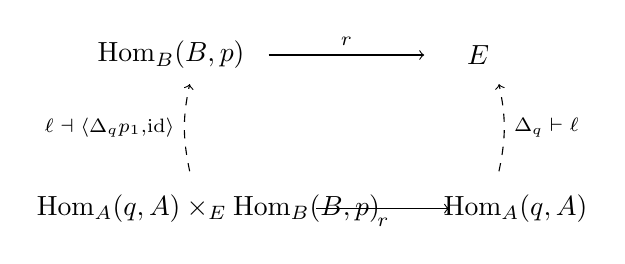
\begin{tikzpicture}[x=1.5em,y=1.5em]
  \node (Hom) at (0,2.2) {$\mathrm{Hom}_{B}(B,p)$};
  \node (E)   at (7.4,2.2) {$E$};
  \node (P)   at (0.9,-1.5)
    {$\mathrm{Hom}_{A}(q,A)\times_{E}\mathrm{Hom}_{B}(B,p)$};
  \node (HomA) at (8.3,-1.5) {$\mathrm{Hom}_{A}(q,A)$};
  \draw[->] (2.35,2.2) -- node[above]{$\scriptstyle r$} (6.1,2.2);
  \draw[->] (3.5,-1.5) -- node[below]{$\scriptstyle r$} (6.7,-1.5);
  \draw[->,dashed] (0.45,-0.6) to[bend left=12] node[left,pos=0.5]{$\scriptstyle\ell\;\dashv\;\langle\Delta_{q}p_{1},\mathrm{id}\rangle$} (0.45,1.5);
  \draw[->,dashed] (7.9,-0.6) to[bend right=12] node[right,pos=0.5]{$\scriptstyle\Delta_{q}\;\vdash\;\ell$} (7.9,1.5);
\end{tikzpicture}
\end{center}
定义了一个同构。这证明了 (i) 蕴涵 (iii)。

反之，假设 (iii)。由\cref{lem:cartesian-on-the-right}与%
\cref{cor:cartesian-cocartesian-conditions}，我们从其中两个伴随得出：%
\trFunctor{}
\begin{center}
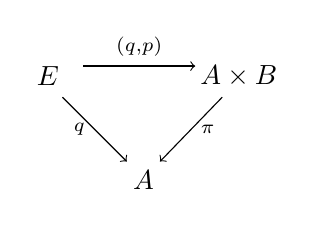
\begin{tikzpicture}[x=1.5em,y=1.5em]
  \node (E)  at (0,1.3) {$E$};
  \node (AB) at (4.6,1.3) {$A\times B$};
  \node (A)  at (2.3,-1.2) {$A$};
  \draw[->] (0.85,1.55) -- node[above]{$\scriptstyle(q,p)$} (3.55,1.55);
  \draw[->] (0.35,0.8) -- node[left,pos=0.5]{$\scriptstyle q$} (1.9,-0.75);
  \draw[->] (4.2,0.8) -- node[right,pos=0.5]{$\scriptstyle\pi$} (2.7,-0.75);
\end{tikzpicture}
\end{center}
\begingroup\emergencystretch=3em\sloppy
落在 $\mathrm{co}\mathcal{C}\mathit{art}(\mathcal{K})_{/A}$ 之中，并定义了
$\mathcal{K}_{/A}$ 里的一条\trCartesianFibration{}；
它也定义 $\mathrm{co}\mathcal{C}\mathit{art}(\mathcal{K})_{/A}$ 中的一条\trCartesianFibration，
当且仅当右伴随 $r$ 是从 $qp_{1}\colon\mathrm{Hom}_{B}(B,p)\twoheadrightarrow A$
到 $q\colon E\twoheadrightarrow A$
的一个\trCartesianFunctor{}（定理 5.2.8(iii)）；回忆包含
$\mathrm{co}\mathcal{C}\mathit{art}(\mathcal{K})_{/A}\hookrightarrow\mathcal{K}_{/A}$
在正维数箭头上是满的，因此在单位与余单位上没有可比较的条件。
由定理 5.3.4(iii)，这由对应 $\ell r\cong r\ell$ 的可逆性得出。
如此我们便看到 (iii) 蕴涵 (i)。
\endgroup

于是，我们已经证明：条件 (i) 等价于 (iii)——后者断言在 $\mathcal{K}_{/A\times B}$
中存在诸伴随，使得实线箭头图的所有对应都是同构。将这个论证对偶化，即可见 (iii)
等价于条件 (ii)。

最后，(iii) 与 (iv) 等价：因为 (iii) 中诸左伴随的存在性等价于该跨度左侧余
笛卡尔，诸右伴随的存在性等价于右侧笛卡尔，而笛卡尔提升与余笛卡尔提升的相容性
条件正是同构 $\ell r\cong r\ell$ 的含义。
\end{proof}

双侧纤维化的内部刻画有一个熟悉的推论：

\begin{corollary}\label{cor:two-sided-fibration-retract}
任何在 $A\times B$ 之上等价于某个\trTwoSidedFibration{}
$(q,p)\colon E\twoheadrightarrow A\times B$ 的\trTwoSidedIsofibration
$(a,b)\colon X\twoheadrightarrow A\times B$，都是一个\trTwoSidedFibration{}。
\end{corollary}

\begin{proof}
\cref{thm:two-sided-fibration}(iii) 的断言在\trFiberedEquivalence{}下不变。
\end{proof}

\cref{thm:two-sided-fibration}可用于确立一个涉及定义 1.1.4 之%
\trOrdinalCategory{}的重要例子族。

\begin{proposition}\label{prop:An-two-sided-fibration}
对任意\trInfinityCategory{} $A$ 与任意 $n\geq 2$，\trTwoSidedIsofibration
$A\xleftarrow{p_{n-1}}A^{n}\xrightarrow{p_{0}}A$ 定义了一个\trTwoSidedFibration{}。
\end{proposition}

这一结果是命题 5.5.11 及其对偶的推广，而其证明使用了类似的想法。

\begin{proof}
我们使用\cref{thm:two-sided-fibration}(iii)。与在\trInitial{}对象处的求值
$p_{0}\colon A^{\mathbb{n}}\to A$ 相关联的右表示\trCommaInfinityCategory{}由
如下拉回构造
\begin{center}
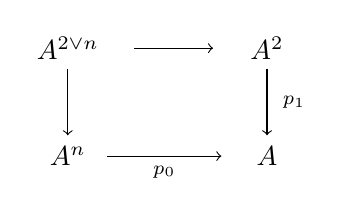
\begin{tikzpicture}[x=1.5em,y=1.5em]
  \node (A2vn) at (0,1.3) {$A^{2\vee\mathbb{n}}$};
  \node (A2)   at (4.8,1.3) {$A^{2}$};
  \node (An)   at (0,-1.3) {$A^{\mathbb{n}}$};
  \node (A)    at (4.8,-1.3) {$A$};
  \draw[->] (1.6,1.3) -- (3.5,1.3);
  \draw[->] (0,0.8) -- (0,-0.8);
  \node at (0.55,0.75) {$\scriptstyle\llcorner$};
  \draw[->] (4.8,0.8) -- (4.8,-0.8);
  \node at (5.45,0) {$\scriptstyle p_{1}$};
  \draw[->] (0.95,-1.3) -- node[below]{$\scriptstyle p_{0}$} (3.7,-1.3);
\end{tikzpicture}
\end{center}
它在诸\trEndpointEvaluation{}映射之下等价于
$(p_{n},p_{0})\colon A^{\mathbb{n}+\mathbb{1}}\twoheadrightarrow A\times A$。
检验 $(p_{n-1},p_{0})\colon A^{\mathbb{n}}\twoheadrightarrow A\times A$ 是否
右侧笛卡尔的典范\trFunctor{}，由沿\trEpimorphism{}
$\sigma^{0}\colon\mathbb{n}+\mathbb{1}\to\mathbb{n}$ 的限制给出，后者把
$\mathbb{n}+\mathbb{1}$ 中的对象 $0,1$ 送到 $\mathbb{n}$ 中的 $0$。该函子在诸%
\trEndpointInclusion{}之下容有一个左伴随
\begin{center}
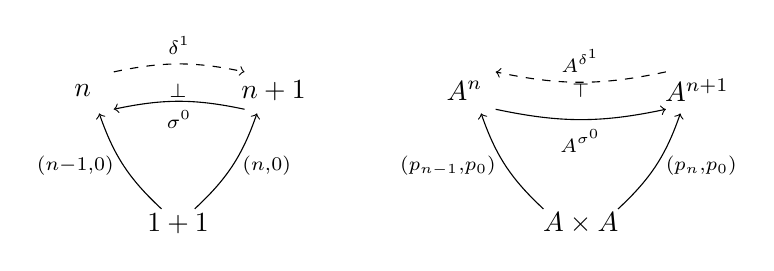
\begin{tikzpicture}[x=1.5em,y=1.5em]
  \node (n)  at (0,1.4) {$\mathbb{n}$};
  \node (n1) at (4.6,1.4) {$\mathbb{n}+\mathbb{1}$};
  \node (oo) at (2.3,-1.8) {$1+1$};
  \draw[->,dashed] (0.75,1.85) to[bend left=12] node[above,pos=0.5]{$\scriptstyle\delta^{1}$} (3.9,1.85);
  \node at (2.3,1.4) {$\scriptstyle\perp$};
  \draw[->] (3.9,0.95) to[bend right=12] node[below,pos=0.5]{$\scriptstyle\sigma^{0}$} (0.75,0.95);
  \draw[->] (1.9,-1.45) to[bend left=14] node[left,pos=0.5]{$\scriptstyle(n-1,0)$} (0.4,0.85);
  \draw[->] (2.7,-1.45) to[bend right=14] node[right,pos=0.5]{$\scriptstyle(n,0)$} (4.2,0.85);
  \node at (7.0,1.4) {$\twoheadrightarrow$};
  \begin{scope}[shift={(9.2,0)}]
  \node (An)  at (0,1.4) {$A^{\mathbb{n}}$};
  \node (An1) at (5.6,1.4) {$A^{\mathbb{n}+\mathbb{1}}$};
  \node (AA)  at (2.8,-1.8) {$A\times A$};
  \draw[->,dashed] (4.85,1.85) to[bend left=12] node[above,pos=0.5]{$\scriptstyle A^{\delta^{1}}$} (0.75,1.85);
  \node at (2.8,1.4) {$\scriptstyle\top$};
  \draw[->] (0.75,0.95) to[bend right=12] node[below,pos=0.5]{$\scriptstyle A^{\sigma^{0}}$} (4.85,0.95);
  \draw[->] (1.9,-1.45) to[bend left=14] node[left,pos=0.5]{$\scriptstyle(p_{n-1},p_{0})$} (0.4,0.85);
  \draw[->] (3.7,-1.45) to[bend right=14] node[right,pos=0.5]{$\scriptstyle(p_{n},p_{0})$} (5.2,0.85);
  \end{scope}
\end{tikzpicture}
\end{center}
如此便给出了上方左图所示的所求纤维化右伴随。

对偶的论证表明 $(p_{n-1},p_{0})\colon A^{\mathbb{n}}\twoheadrightarrow A\times A$ 是左侧余笛卡尔的。最后的条件要求：由诸\trDegeneracyOperator{}定义的交换方块的对应
\begin{center}
\begin{tikzpicture}[x=1.5em,y=1.5em]
  \node (n)   at (0,2.2) {$\mathbb{n}$};
  \node (n1t) at (4.6,2.2) {$\mathbb{n}+\mathbb{1}$};
  \node (n1b) at (0,-1.6) {$\mathbb{n}+\mathbb{1}$};
  \node (n2)  at (4.6,-1.6) {$\mathbb{n}+2$};
  \draw[->,dashed] (0.75,2.65) to[bend left=12] node[above,pos=0.5]{$\scriptstyle\delta^{1}$} (3.9,2.65);
  \node at (2.3,2.2) {$\scriptstyle\perp$};
  \draw[->] (3.9,1.75) to[bend right=12] node[below,pos=0.5]{$\scriptstyle\sigma^{0}$} (0.75,1.75);
  \draw[->] (3.9,-1.15) to[bend right=12] node[above,pos=0.5]{$\scriptstyle\sigma^{0}$} (0.75,-1.15);
  \node at (2.3,-1.6) {$\scriptstyle\top$};
  \draw[->,dashed] (0.75,-2.05) to[bend left=12] node[below,pos=0.5]{$\scriptstyle\delta^{1}$} (3.9,-2.05);
  \draw[->,dashed] (-0.55,1.45) to[bend left=14] node[left,pos=0.5]{$\scriptstyle\delta^{n}\;\dashv\;\sigma^{n}$} (-0.55,0.15);
  \draw[->,dashed] (5.15,0.15) to[bend left=14] node[right,pos=0.5]{$\scriptstyle\sigma^{n+1}\;\dashv\;\delta^{n+1}$} (5.15,1.45);
\end{tikzpicture}
\end{center}
是同构，编码了诸单纯恒等式中我们熟悉的一个。\cref{thm:two-sided-fibration}(iii)%
中的方块可通过应用 $A^{(-)}$ 而得到。
\end{proof}

我们把对双侧纤维化这一类对象的诸封闭性质的进一步讨论推迟到下一节，在那里我们
将部署宇宙论的论证来精简它们的证明。这些观察使我们得以进一步扩充我们的例子族。

为那一工作做准备，我们考虑双侧纤维化之间的保结构态射，证明%
\cref{thm:two-sided-fibration}的一个相对类比：

\begin{proposition}\label{prop:map-of-spans}
对于 ∞-宇宙 $\mathcal{K}$ 中一对从 $A$ 到 $B$ 的双侧纤维化之间的如下跨度映射
\begin{center}
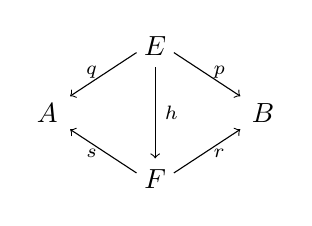
\begin{tikzpicture}[x=1.5em,y=1.5em]
  \node (E) at (2.6,1.6) {$E$};
  \node (A) at (0,0) {$A$};
  \node (B) at (5.2,0) {$B$};
  \node (F) at (2.6,-1.6) {$F$};
  \draw[->] (2.15,1.45) -- node[above,left,pos=0.45]{$\scriptstyle q$} (0.55,0.4);
  \draw[->] (3.05,1.45) -- node[above,right,pos=0.45]{$\scriptstyle p$} (4.65,0.4);
  \draw[->] (2.6,1.1) -- node[right,pos=0.5]{$\scriptstyle h$} (2.6,-1.1);
  \draw[->] (2.15,-1.45) -- node[below,left,pos=0.45]{$\scriptstyle s$} (0.55,-0.4);
  \draw[->] (3.05,-1.45) -- node[below,right,pos=0.45]{$\scriptstyle r$} (4.65,-0.4);
\end{tikzpicture}
\end{center}
下列诸条等价：
\begin{enumerate}[label=(\roman*)]
\item $h$ 定义了 $\mathrm{co}\mathcal{C}\mathit{art}(\mathcal{K})_{/A}$ 中诸%
\trCartesianFibration{}之间的一个\trCartesianFunctor{}。
\item $h$ 定义了 $\mathcal{C}art(\mathcal{K})_{/B}$ 中诸%
\trCocartesianFibration{}之间的一个\trCartesianFunctor{}。
\item 诸典范同构
\begin{center}
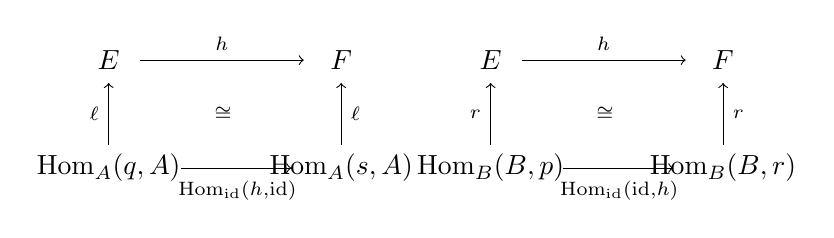
\begin{tikzpicture}[x=1.5em,y=1.5em]
  \node (E1) at (0,1.3) {$E$};
  \node (F1) at (5.6,1.3) {$F$};
  \node (H1) at (0,-1.3) {$\mathrm{Hom}_{A}(q,A)$};
  \node (H2) at (5.6,-1.3) {$\mathrm{Hom}_{A}(s,A)$};
  \draw[->] (0.75,1.3) -- node[above]{$\scriptstyle h$} (4.7,1.3);
  \draw[->] (0,-0.75) -- node[left]{$\scriptstyle\ell$} (0,0.75);
  \draw[->] (5.6,-0.75) -- node[right]{$\scriptstyle\ell$} (5.6,0.75);
  \draw[->] (1.75,-1.3) -- (4.4,-1.3);
  \node at (3.1,-1.85) {$\scriptstyle\mathrm{Hom}_{\mathrm{id}}(h,\mathrm{id})$};
  \node at (2.8,0) {$\scriptstyle\cong\,\curvearrowleft$};
  \begin{scope}[shift={(9.2,0)}]
  \node (E2) at (0,1.3) {$E$};
  \node (F2) at (5.6,1.3) {$F$};
  \node (H3) at (0,-1.3) {$\mathrm{Hom}_{B}(B,p)$};
  \node (H4) at (5.6,-1.3) {$\mathrm{Hom}_{B}(B,r)$};
  \draw[->] (0.75,1.3) -- node[above]{$\scriptstyle h$} (4.7,1.3);
  \draw[->] (0,-0.75) -- node[left]{$\scriptstyle r$} (0,0.75);
  \draw[->] (5.6,-0.75) -- node[right]{$\scriptstyle r$} (5.6,0.75);
  \draw[->] (1.75,-1.3) -- (4.4,-1.3);
  \node at (3.1,-1.85) {$\scriptstyle\mathrm{Hom}_{\mathrm{id}}(\mathrm{id},h)$};
  \node at (2.8,0) {$\scriptstyle\cong\,\curvearrowleft$};
  \end{scope}
\end{tikzpicture}
\end{center}
的对应定义了 $\mathcal{K}_{/A\times B}$ 中的同构。
\item 在 $\mathcal{K}$ 中，$h$ 定义了余笛卡尔纤维化 $q$ 与 $s$ 之间的一个笛卡尔
函子，以及笛卡尔纤维化 $p$ 与 $r$ 之间的一个\trCartesianFunctor{}。
\end{enumerate}
当这些等价条件被满足时，该跨度映射就定义了从 $A$ 到 $B$ 的双侧纤维化之间的一个%
\textbf{\trCartesianFunctor}（cartesian functor）。
\end{proposition}

\begin{proof}
由定理 5.3.4(iii)，条件 (iv) 等价于要求 (iii) 中所示的两个对应分别是
$\mathcal{K}_{/A}$ 与 $\mathcal{K}_{/B}$ 中的同构。但由于这些跨度是从 $A$ 到
$B$ 的双侧纤维化，且 $h$ 是 $A\times B$ 之上的映射，这两个%
\trNaturalTransformation{}都位于 $\mathcal{K}_{/A\times B}$ 之中。由命题
3.6.2，如果这些\trNaturalTransformation{}在 $\mathcal{K}_{/A}$ 与
$\mathcal{K}_{/B}$ 中容有逆，那么这些逆变换就提升为 $\mathcal{K}_{/A\times B}$
中的一个逆同构。这证明了 (iv) 等价于 (iii)。

我们接下来证明 (i) 等价于 (iii)。(ii) 与 (iii) 之等价的证明是对偶的。要像
(i) 中那样断言映射
\begin{center}
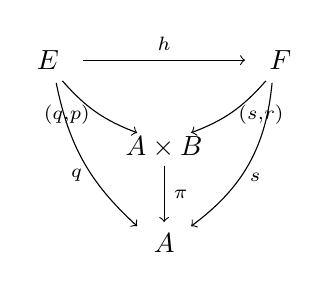
\begin{tikzpicture}[x=1.5em,y=1.5em]
  \node (E)  at (0,2.4) {$E$};
  \node (F)  at (5.6,2.4) {$F$};
  \node (AB) at (2.8,0.3) {$A\times B$};
  \node (A)  at (2.8,-2.0) {$A$};
  \draw[->] (0.85,2.4) -- node[above]{$\scriptstyle h$} (4.75,2.4);
  \draw[->] (0.35,1.9) to[bend right=14] node[left,pos=0.55]{$\scriptstyle(q,p)$} (2.15,0.65);
  \draw[->] (5.25,1.9) to[bend left=14] node[right,pos=0.55]{$\scriptstyle(s,r)$} (3.45,0.65);
  \draw[->] (0.2,1.85) to[bend right=18] node[left,pos=0.6]{$\scriptstyle q$} (2.15,-1.6);
  \draw[->] (5.4,1.85) to[bend left=24] node[right,pos=0.6]{$\scriptstyle s$} (3.45,-1.6);
  \draw[->] (2.8,-0.15) -- node[right,pos=0.5]{$\scriptstyle\pi$} (2.8,-1.5);
\end{tikzpicture}
\end{center}
定义了 $\mathrm{co}\mathcal{C}\mathit{art}(\mathcal{K})_{/A}$ 中诸%
\trCartesianFibration{}之间的一个\trCartesianFunctor{}，首先意味着对应
\begin{center}
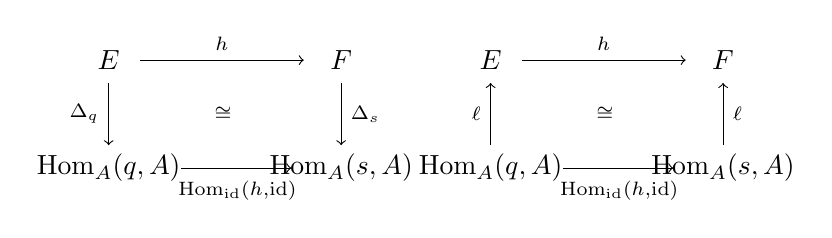
\begin{tikzpicture}[x=1.5em,y=1.5em]
  \node (E1) at (0,1.3) {$E$};
  \node (F1) at (5.6,1.3) {$F$};
  \node (H1) at (0,-1.3) {$\mathrm{Hom}_{A}(q,A)$};
  \node (H2) at (5.6,-1.3) {$\mathrm{Hom}_{A}(s,A)$};
  \draw[->] (0.75,1.3) -- node[above]{$\scriptstyle h$} (4.7,1.3);
  \draw[->] (0,0.75) -- node[left]{$\scriptstyle\Delta_{q}$} (0,-0.75);
  \draw[->] (5.6,0.75) -- node[right]{$\scriptstyle\Delta_{s}$} (5.6,-0.75);
  \draw[->] (1.75,-1.3) -- (4.4,-1.3);
  \node at (3.1,-1.85) {$\scriptstyle\mathrm{Hom}_{\mathrm{id}}(h,\mathrm{id})$};
  \node at (2.8,0) {$\scriptstyle\cong\,\curvearrowleft$};
  \node at (7.6,0) {$\rightsquigarrow$};
  \begin{scope}[shift={(9.2,0)}]
  \node (E2) at (0,1.3) {$E$};
  \node (F2) at (5.6,1.3) {$F$};
  \node (H3) at (0,-1.3) {$\mathrm{Hom}_{A}(q,A)$};
  \node (H4) at (5.6,-1.3) {$\mathrm{Hom}_{A}(s,A)$};
  \draw[->] (0.75,1.3) -- node[above]{$\scriptstyle h$} (4.7,1.3);
  \draw[->] (0,-0.75) -- node[left]{$\scriptstyle\ell$} (0,0.75);
  \draw[->] (5.6,-0.75) -- node[right]{$\scriptstyle\ell$} (5.6,0.75);
  \draw[->] (1.75,-1.3) -- (4.4,-1.3);
  \node at (3.1,-1.85) {$\scriptstyle\mathrm{Hom}_{\mathrm{id}}(h,\mathrm{id})$};
  \node at (2.8,0) {$\scriptstyle\cong\,\curvearrowleft$};
  \end{scope}
\end{tikzpicture}
\end{center}
定义了 $\mathcal{K}_{/A}$ 中的一个同构——因为 $h$ 在 $A$ 之上定义了余笛卡尔
纤维化 $q$ 与 $s$ 之间的一个\trCartesianFunctor{}；其次意味着对应
\begin{center}
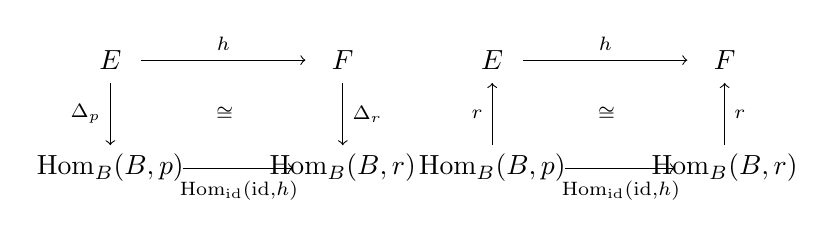
\begin{tikzpicture}[x=1.5em,y=1.5em]
  \node (E1) at (0,1.3) {$E$};
  \node (F1) at (5.6,1.3) {$F$};
  \node (H1) at (0,-1.3) {$\mathrm{Hom}_{B}(B,p)$};
  \node (H2) at (5.6,-1.3) {$\mathrm{Hom}_{B}(B,r)$};
  \draw[->] (0.75,1.3) -- node[above]{$\scriptstyle h$} (4.7,1.3);
  \draw[->] (0,0.75) -- node[left]{$\scriptstyle\Delta_{p}$} (0,-0.75);
  \draw[->] (5.6,0.75) -- node[right]{$\scriptstyle\Delta_{r}$} (5.6,-0.75);
  \draw[->] (1.75,-1.3) -- (4.4,-1.3);
  \node at (3.1,-1.85) {$\scriptstyle\mathrm{Hom}_{\mathrm{id}}(\mathrm{id},h)$};
  \node at (2.8,0) {$\scriptstyle\cong\,\curvearrowleft$};
  \node at (7.6,0) {$\rightsquigarrow$};
  \begin{scope}[shift={(9.2,0)}]
  \node (E2) at (0,1.3) {$E$};
  \node (F2) at (5.6,1.3) {$F$};
  \node (H3) at (0,-1.3) {$\mathrm{Hom}_{B}(B,p)$};
  \node (H4) at (5.6,-1.3) {$\mathrm{Hom}_{B}(B,r)$};
  \draw[->] (0.75,1.3) -- node[above]{$\scriptstyle h$} (4.7,1.3);
  \draw[->] (0,-0.75) -- node[left]{$\scriptstyle r$} (0,0.75);
  \draw[->] (5.6,-0.75) -- node[right]{$\scriptstyle r$} (5.6,0.75);
  \draw[->] (1.75,-1.3) -- (4.4,-1.3);
  \node at (3.1,-1.85) {$\scriptstyle\mathrm{Hom}_{\mathrm{id}}(\mathrm{id},h)$};
  \node at (2.8,0) {$\scriptstyle\cong\,\curvearrowleft$};
  \end{scope}
\end{tikzpicture}
\end{center}
是 $(\mathrm{co}\mathcal{C}\mathit{art}(\mathcal{K})_{/A})_{/\pi}$ 中的一个同构。由于
这些跨度是双侧纤维化，且 $h$ 是 $A\times B$ 之上的映射，第一对对应位于
$\mathcal{K}_{/A\times B}$ 之中。而由于包含
$(\mathrm{co}\mathcal{C}\mathit{art}(\mathcal{K})_{/A})_{/\pi}\hookrightarrow\mathcal{K}_{/A\times B}$ 在正维数箭头上是满的，要求第二对对应是
$(\mathrm{co}\mathcal{C}\mathit{art}(\mathcal{K})_{/A})_{/\pi}$ 中的同构，就等价于要求
同一条件在 $\mathcal{K}_{/A\times B}$ 中成立。这就证明了与 (iii) 的等价。
\end{proof}


这由\cref{thm:two-sided-fibration}与\cref{prop:map-of-spans}的内部刻画可得。

\begin{corollary}\label{cor:cosmological-preserves-two-sided}
任何宇宙论\trFunctor{}都保持\trTwoSidedFibration{}以及它们之间的\trCartesianFunctor{}。
\end{corollary}

\begin{proof}
由命题 1.3.4(vi)，任何宇宙论\trFunctor{} $F\colon\mathcal{K}\to\mathcal{L}$
对 $\mathcal{K}$ 中任意一对\trInfinityCategory{} $A$ 与 $B$ 都诱导一个宇宙论%
\trFunctor{} $F'\colon\mathcal{K}_{/A\times B}\to\mathcal{L}_{/FA\times FB}$。
该\trFunctor{}保持\cref{thm:two-sided-fibration}(iii) 的诸\trFiberedAdjunction{}与可逆
对应。于是
$F\colon\mathcal{K}\to\mathcal{L}$ 保持双侧纤维化；类似地，任何宇宙论%
\trFunctor{}都保持\cref{prop:map-of-spans}(iii) 的可逆对应。
\end{proof}


\subsection*{练习}

\begin{exercise}\label{ex:product-projection-span}
证明：对任意\trInfinityCategory{} $A$ 与 $B$，乘积投影跨度
$A\xleftarrow{\pi}A\times B\xrightarrow{\pi}B$ 定义了一个\trTwoSidedFibration{}。
\end{exercise}

\begin{exercise}\label{ex:two-sided-from-terminal}
证明：
\begin{enumerate}[label=(\roman*)]
\item \trTwoSidedIsofibration $1\xleftarrow{!}E\xrightarrow{p}B$ 定义了从 $1$ 到 $B$
的一个\trTwoSidedFibration{}，当且仅当 $p\colon E\twoheadrightarrow B$ 是一条%
\trCartesianFibration{}。
\item 如下所示的跨度映射定义了双侧纤维化之间的一个\trCartesianFunctor{}，当且仅当
$h\colon E\to F$ 定义了从 $p$ 到 $q$ 的一个\trCartesianFunctor{}。
\end{enumerate}
\begin{center}
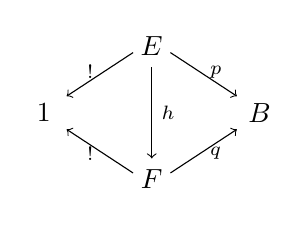
\begin{tikzpicture}[x=1.5em,y=1.5em]
  \node (E) at (2.6,1.6) {$E$};
  \node (o) at (0,0) {$1$};
  \node (B) at (5.2,0) {$B$};
  \node (F) at (2.6,-1.6) {$F$};
  \draw[->] (2.15,1.45) -- node[above,left,pos=0.45]{$\scriptstyle !$} (0.55,0.4);
  \draw[->] (3.05,1.45) -- node[above,right,pos=0.45]{$\scriptstyle p$} (4.65,0.4);
  \draw[->] (2.6,1.1) -- node[right,pos=0.5]{$\scriptstyle h$} (2.6,-1.1);
  \draw[->] (2.15,-1.45) -- node[below,left,pos=0.45]{$\scriptstyle !$} (0.55,-0.4);
  \draw[->] (3.05,-1.45) -- node[below,right,pos=0.45]{$\scriptstyle q$} (4.65,-0.4);
\end{tikzpicture}
\end{center}
\end{exercise}

\begin{exercise}\label{ex:mate-fibered-iso}
设 $A\xleftarrow{q}E\xrightarrow{p}B$ 与 $A\xleftarrow{s}F\xrightarrow{r}B$
是双侧纤维化，且 $\alpha\colon h\cong h'$ 是一个纤维化自然同构
\begin{center}
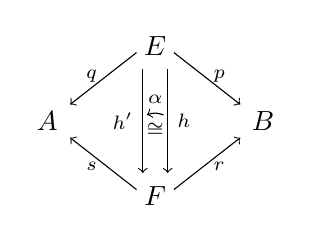
\begin{tikzpicture}[x=1.5em,y=1.5em]
  \node (E) at (2.6,1.8) {$E$};
  \node (A) at (0,0) {$A$};
  \node (B) at (5.2,0) {$B$};
  \node (F) at (2.6,-1.8) {$F$};
  \draw[->] (2.15,1.65) -- node[above,left,pos=0.45]{$\scriptstyle q$} (0.55,0.4);
  \draw[->] (3.05,1.65) -- node[above,right,pos=0.45]{$\scriptstyle p$} (4.65,0.4);
  \draw[->] (2.9,1.25) -- node[right,pos=0.5]{$\scriptstyle h$} (2.9,-1.25);
  \draw[->] (2.3,1.25) -- node[left,pos=0.5]{$\scriptstyle h'$} (2.3,-1.25);
  \draw[->] (2.8,0.15) to[bend right=20] node[above,pos=0.5]{$\scriptstyle\alpha$} node[below,pos=0.5]{$\scriptstyle\cong$} (2.4,0.15);
  \draw[->] (2.15,-1.65) -- node[below,left,pos=0.45]{$\scriptstyle s$} (0.55,-0.4);
  \draw[->] (3.05,-1.65) -- node[below,right,pos=0.45]{$\scriptstyle r$} (4.65,-0.4);
\end{tikzpicture}
\end{center}
使得 $r\alpha=\mathrm{id}_{p}$ 且 $s\alpha=\mathrm{id}_{q}$；特别地，$h$ 与
$h'$ 各自定义了一个跨度映射。证明：$h$ 是一个\trCartesianFunctor{}，当且仅当 $h'$ 是一个%
\trCartesianFunctor{}。
\end{exercise}
